Consider the equilateral triangle formed by connecting the centers of the three circles positions at the far east/west/north positions. The center of the triangle --- the point where the three bisectors intersect --- is also the center of the large circle. Let $a$ denote the side length of the triangle. Let $x$ denote the distance from one vertex to the center of the triangle. The height of the triangle is $x+y$. See the figure below. 
\begin{figure}[H]
\centering
\includegraphics[width=0.45\linewidth,page=2]{circles-in-pyramid}%
\includegraphics[width=0.45\linewidth,page=3]{circles-in-pyramid}
\end{figure}
Let $R$ denote the radius of the larger circle. Then $R=x+r$. We want to express $x$ in terms of $r$ and $n$. To do this, we first express $x$ in terms of $a$ and then express $a$ in terms of $r$ and $n$. The relation between $x$ and $a$ for an equilateral triangle is well known; it is not difficult to calculate it by applying the Pythagorean theorem (see below). We state it here: 
\begin{align*}
x = \frac{\sqrt{3}a}{3}
\end{align*}
We can express $a$ in terms of $r$ and $n$ as follows. The circle's centers are a distance $r$ from the circle. The distance between two centers is equal to the diameter multiplied by the number of circles, or $n-2$. This gives a side length of $r + 2r(n-2) + r$ (adding lengths from one end to the other) and thus
\begin{align*}
a =  2r(n-1)
\end{align*}
Substituting back into $x$ gives
\begin{align*}
x = \frac{2\sqrt{3}(n-1)r}{3}
\end{align*}
The radius of the larger circle $R=r+x$ is therefore 
\begin{align*}
R = \frac{\left(3+2\sqrt{3}(n-1)\right)r}{3}
\end{align*}

The pyramid's base has $n$ circles, the next row above $n-1$, the one above $n-2$, and so on until the top row with $1$ circle. The total number of circles is therefore:
\begin{align*}
n + (n-1) + (n-2) + \ldots + 1
  = \frac{n(n+1)}{2}
\end{align*}

The area of one small circle is $\pi r^2$. The ratio of the areas occupied by the small circles to the area of the larger circle is:
\begin{align*}
\frac{\dfrac{n(n+1)}{2} \pi r^2}{\pi R^2}
 & = 
\frac{\dfrac{n(n+1)}{2}}{\dfrac{\left(3+2\sqrt{3}(n-1)\right)^2}{3^2}}\\[1em]
 & = 
\dfrac{9n(n+1)}{2\left(3+2\sqrt{3}(n-1)\right)^2}\\[1em]
 & = 
\dfrac{3n(n+1)}{2\left(3+4\sqrt{3}(n-1)+4(n-1)^2\right)}
\end{align*}

How does this ratio depend on $n$? The figure below shows the percentage of the larger circle's area filled by the small circles for several values of $n$. 
\begin{figure}[H]
\centering
\includegraphics[width=\linewidth,page=6]{circles-in-pyramid}
\end{figure}
As $n$ gets larger, the ratio tends to:
\begin{align*}
\frac{3n(n+1)}{8(n-1)^2} \rightarrow \frac{3}{8}
~\text{as}~n\rightarrow\infty
\end{align*}
How does this compare to the ratio of the area of the triangle to the area of the larger circle? The area of the triangle is:
\begin{align*}
%\frac{a(x+y)}{2} = 
\frac{\sqrt{3}a^2}{4}
  = \sqrt{3}(n-1)^2r^2
\end{align*}
And therefore the ratio of areas:
\begin{align*}
\frac{\sqrt{3}(n-1)^2r^2}{\dfrac{\pi\left(3+2\sqrt{3}(n-1)\right)^2r^2}{3^2}}
= \frac{3\sqrt{3}(n-1)^2}{\pi\left(3+4\sqrt{3}(n-1)+4(n-1)^2\right)}
\rightarrow \frac{3\sqrt{3}}{4\pi}~\text{as}~n\rightarrow\infty
\end{align*}

In the limit, as the number of smaller circles becomes arbitrarily large, $n\rightarrow\infty$, the area covered by the circles tends to $0.375$, while the area of the triangle is approximately $0.413$, about $10$ percent larger. 

We now show how to calculate $x$ in an equilateral triangle of side length $a$. We first calculate the height of the triangle. Let $h$ denote the height:
\begin{figure}[H]
\centering
\includegraphics[height=5cm,page=7]{circles-in-pyramid}
\end{figure}

Apply the Pythagorean theorem to find the height $h$:
\begin{align*}
& \left(\frac{a}{2}\right)^2 + h^2 = a^2 \\
\Rightarrow 
& h = \frac{\sqrt{3}a}{2}
\end{align*}

Split the height into two parts, $h=x+y$:
\begin{figure}[H]
\centering
\includegraphics[height=5cm,page=3]{circles-in-pyramid}
\end{figure}
Apply the Pythagorean theorem and eliminate $y$ by substituting $y=h-x$:
\begin{align*}
& \left(\frac{a}{2}\right)^2 + y^2 = x^2 \\
\Rightarrow \quad
& \left(\frac{a}{2}\right)^2 + \left(\frac{\sqrt{3}a}{2}-x\right)^2 = x^2 \\
\Rightarrow \quad
& \left(\frac{a}{2}\right)^2 + 3 \left(\frac{a}{2}\right)^2 - \sqrt{3}ax + x^2 = x^2 \\[1em]
\Rightarrow \quad
& x = \dfrac{4\left(\dfrac{a}{2}\right)^2}{\sqrt{3}a} \\[1em]
\Rightarrow \quad
& x = \frac{\sqrt{3}a}{3}
\end{align*}
With $h$ and $x$, we can also calculate $y = \dfrac{\sqrt{3}a}{6}$.
